\documentclass[landscape,final,a0paper,fontscale=0.285]{baposter}

\usepackage{calc}
\usepackage{graphicx}
\usepackage{amsmath}
\usepackage{amssymb}
\usepackage{relsize}
\usepackage{multirow}
\usepackage{rotating}
\usepackage{bm}
\usepackage{url}
\usepackage{colortbl}

\usepackage{graphicx}
\usepackage{multicol}

%\usepackage{times}
%\usepackage{helvet}
%\usepackage{bookman}
\usepackage{palatino}

\makeatletter
\bibliographystyle{utf8gost71u}     % Оформляем библиографию по ГОСТ 7.1 (ГОСТ Р 7.0.11-2011, 5.6.7)
\renewcommand{\@biblabel}[1]{#1.}   % Заменяем библиографию с квадратных скобок на точку

\bibliographystyle{srt}
\makeatother

\newcommand{\captionfont}{\footnotesize}

\graphicspath{{images/}{../images/}}
\usetikzlibrary{calc}

\newcommand{\SET}[1]  {\ensuremath{\mathcal{#1}}}
\newcommand{\MAT}[1]  {\ensuremath{\boldsymbol{#1}}}
\newcommand{\VEC}[1]  {\ensuremath{\boldsymbol{#1}}}
\newcommand{\Video}{\SET{V}}
\newcommand{\video}{\VEC{f}}
\newcommand{\track}{x}
\newcommand{\Track}{\SET T}
\newcommand{\LMs}{\SET L}
\newcommand{\lm}{l}
\newcommand{\PosE}{\SET P}
\newcommand{\posE}{\VEC p}
\newcommand{\negE}{\VEC n}
\newcommand{\NegE}{\SET N}
\newcommand{\Occluded}{\SET O}
\newcommand{\occluded}{o}

%%%%%%%%%%%%%%%%%%%%%%%%%%%%%%%%%%%%%%%%%%%%%%%%%%%%%%%%%%%%%%%%%%%%%%%%%%%%%%%%
%%%% Some math symbols used in the text
%%%%%%%%%%%%%%%%%%%%%%%%%%%%%%%%%%%%%%%%%%%%%%%%%%%%%%%%%%%%%%%%%%%%%%%%%%%%%%%%

%%%%%%%%%%%%%%%%%%%%%%%%%%%%%%%%%%%%%%%%%%%%%%%%%%%%%%%%%%%%%%%%%%%%%%%%%%%%%%%%
% Multicol Settings
%%%%%%%%%%%%%%%%%%%%%%%%%%%%%%%%%%%%%%%%%%%%%%%%%%%%%%%%%%%%%%%%%%%%%%%%%%%%%%%%
\setlength{\columnsep}{1.5em}
\setlength{\columnseprule}{0mm}

%%%%%%%%%%%%%%%%%%%%%%%%%%%%%%%%%%%%%%%%%%%%%%%%%%%%%%%%%%%%%%%%%%%%%%%%%%%%%%%%
% Save space in lists. Use this after the opening of the list
%%%%%%%%%%%%%%%%%%%%%%%%%%%%%%%%%%%%%%%%%%%%%%%%%%%%%%%%%%%%%%%%%%%%%%%%%%%%%%%%
\newcommand{\compresslist}{%
\setlength{\itemsep}{1pt}%
\setlength{\parskip}{0pt}%
\setlength{\parsep}{0pt}%
}

%%%%%%%%%%%%%%%%%%%%%%%%%%%%%%%%%%%%%%%%%%%%%%%%%%%%%%%%%%%%%%%%%%%%%%%%%%%%%%
%%% Begin of Document
%%%%%%%%%%%%%%%%%%%%%%%%%%%%%%%%%%%%%%%%%%%%%%%%%%%%%%%%%%%%%%%%%%%%%%%%%%%%%%

\begin{document}

%%%%%%%%%%%%%%%%%%%%%%%%%%%%%%%%%%%%%%%%%%%%%%%%%%%%%%%%%%%%%%%%%%%%%%%%%%%%%%
%%% Here starts the poster
%%%---------------------------------------------------------------------------
%%% Format it to your taste with the options
%%%%%%%%%%%%%%%%%%%%%%%%%%%%%%%%%%%%%%%%%%%%%%%%%%%%%%%%%%%%%%%%%%%%%%%%%%%%%%
% Define some colors

%\definecolor{lightblue}{cmyk}{0.83,0.24,0,0.12}
\definecolor{lightblue}{rgb}{0.145,0.6666,1}

% Draw a video
\newlength{\FSZ}
\newcommand{\drawvideo}[3]{% [0 0.25 0.5 0.75 1 1.25 1.5]
   \noindent\pgfmathsetlength{\FSZ}{\linewidth/#2}
   \begin{tikzpicture}[outer sep=0pt,inner sep=0pt,x=\FSZ,y=\FSZ]
   \draw[color=lightblue!50!black] (0,0) node[outer sep=0pt,inner sep=0pt,text width=\linewidth,minimum height=0] (video) {\noindent#3};
   \path [fill=lightblue!50!black,line width=0pt] 
     (video.north west) rectangle ([yshift=\FSZ] video.north east) 
    \foreach \x in {1,2,...,#2} {
      {[rounded corners=0.6] ($(video.north west)+(-0.7,0.8)+(\x,0)$) rectangle +(0.4,-0.6)}
    }
;
   \path [fill=lightblue!50!black,line width=0pt] 
     ([yshift=-1\FSZ] video.south west) rectangle (video.south east) 
    \foreach \x in {1,2,...,#2} {
      {[rounded corners=0.6] ($(video.south west)+(-0.7,-0.2)+(\x,0)$) rectangle +(0.4,-0.6)}
    }
;
   \foreach \x in {1,...,#1} {
     \draw[color=lightblue!50!black] ([xshift=\x\linewidth/#1] video.north west) -- ([xshift=\x\linewidth/#1] video.south west);
   }
   \foreach \x in {0,#1} {
     \draw[color=lightblue!50!black] ([xshift=\x\linewidth/#1,yshift=1\FSZ] video.north west) -- ([xshift=\x\linewidth/#1,yshift=-1\FSZ] video.south west);
   }
   \end{tikzpicture}
}

\hyphenation{resolution occlusions}
%%
\begin{poster}%
  % Poster Options
  {
  % Show grid to help with alignment
  grid=false,
  % Column spacing
  colspacing=1em,
  % Color style
  bgColorOne=white,
  bgColorTwo=white,
  borderColor=lightblue,
  headerColorOne=black,
  headerColorTwo=lightblue,
  headerFontColor=white,
  boxColorOne=white,
  boxColorTwo=lightblue,
  % Format of textbox
  textborder=roundedleft,
  % Format of text header
  eyecatcher=true,
  headerborder=closed,
  headerheight=0.1\textheight,
%  textfont=\sc, An example of changing the text font
  headershape=roundedright,
  headershade=shadelr,
  headerfont=\Large\bf\textsc, %Sans Serif
  textfont={\setlength{\parindent}{1.5em}},
  boxshade=plain,
%  background=shade-tb,
  background=plain,
  linewidth=2pt
  }
  % Eye Catcher
  {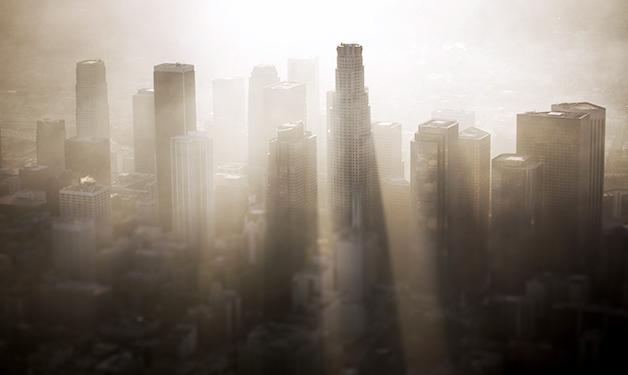
\includegraphics[height=6em]{logo_left}} 
  % Title
  {{\bf\textsc{Air pollutioution - the problem for generation}\vspace{0.5em}} \\ Epigenetic effects of air pollution}
  % Authors
  {\textsc{Team \#5}}
  % University logo
  {% The makebox allows the title to flow into the logo, this is a hack because of the L shaped logo.
    
\includegraphics[height=9.0em]{logo_wsci}
  }

%%%%%%%%%%%%%%%%%%%%%%%%%%%%%%%%%%%%%%%%%%%%%%%%%%%%%%%%%%%%%%%%%%%%%%%%%%%%%%
%%% Now define the boxes that make up the poster
%%%---------------------------------------------------------------------------
%%% Each box has a name and can be placed absolutely or relatively.
%%% The only inconvenience is that you can only specify a relative position 
%%% towards an already declared box. So if you have a box attached to the 
%%% bottom, one to the top and a third one which should be in between, you 
%%% have to specify the top and bottom boxes before you specify the middle 
%%% box.
%%%%%%%%%%%%%%%%%%%%%%%%%%%%%%%%%%%%%%%%%%%%%%%%%%%%%%%%%%%%%%%%%%%%%%%%%%%%%%
    %
    % A coloured circle useful as a bullet with an adjustably strong filling
    \newcommand{\colouredcircle}{%
      \tikz{\useasboundingbox (-0.2em,-0.32em) rectangle(0.2em,0.32em); \draw[draw=black,fill=lightblue,line width=0.03em] (0,0) circle(0.18em);}}

%%%%%%%%%%%%%%%%%%%%%%%%%%%%%%%%%%%%%%%%%%%%%%%%%%%%%%%%%%%%%%%%%%%%%%%%%%%%%%
  \headerbox{Introduction}{name=introduction,column=0,row=0}{
%%%%%%%%%%%%%%%%%%%%%%%%%%%%%%%%%%%%%%%%%%%%%%%%%%%%%%%%%%%%%%%%%%%%%%%%%%%%%%
\begin{itemize} \compresslist
  \item Ambient particulate matter (PM) has been associated with
mortality and morbidity for cardiovascular disease (CVD)
\item MicroRNAs control gene expression at a post-transcriptional
level.
\item Altered microRNAs expression has been reported in
processes related to CVD and PM exposure, e.g. systemic
inflammation, endothelial dysfunction and atherosclerosis.
\end{itemize}
   \vspace{0.3em}
 }

%%%%%%%%%%%%%%%%%%%%%%%%%%%%%%%%%%%%%%%%%%%%%%%%%%%%%%%%%%%%%%%%%%%%%%%%%%%%%%
  \headerbox{Aims/Objectives}{name=contribution,column=0,row=0,below=introduction,above=bottom}{
%%%%%%%%%%%%%%%%%%%%%%%%%%%%%%%%%%%%%%%%%%%%%%%%%%%%%%%%%%%%%%%%%%%%%%%%%%%%%%
   To investigate the association of exposure to ambient articles and blood-leukocyte expression changes in fourteen candidate microRNAs.
   \vspace{0.3em}
  }

%%%%%%%%%%%%%%%%%%%%%%%%%%%%%%%%%%%%%%%%%%%%%%%%%%%%%%%%%%%%%%%%%%%%%%%%%%%%%%
\headerbox{Future works}{name=future_works,column=3,span=1,row=0}{
Lorem ipsum dolor sit amet, consectetur adipisicing elit, sed do eiusmod
tempor incididunt ut labore et dolore magna aliqua. Ut enim ad minim veniam,
quis nostrud exercitation ullamco laboris nisi ut aliquip ex ea commodo
consequat. Duis aute irure dolor in reprehenderit in voluptate velit esse
cillum dolore eu fugiat nulla pariatur. Excepteur sint occaecat cupidatat non
proident, sunt in culpa qui officia deserunt mollit anim id est laborum.  
  %%%%%%%%%%%%%%%%%%%%%%%%%%%%%%%%%%%%%%%%%%%%%%%%%%%%%%%%%%%%%%%%%%%%%%%%%%%%%%
  % \begin{tabular*}{\linewidth}{*{5}{@{}p{0.6\linewidth}@{}}}
  %   {Figure A\hfill{}Figure B\hfill{}}
  % \end{tabular*}
  %   \drawvideo{2}{40}{%
  %      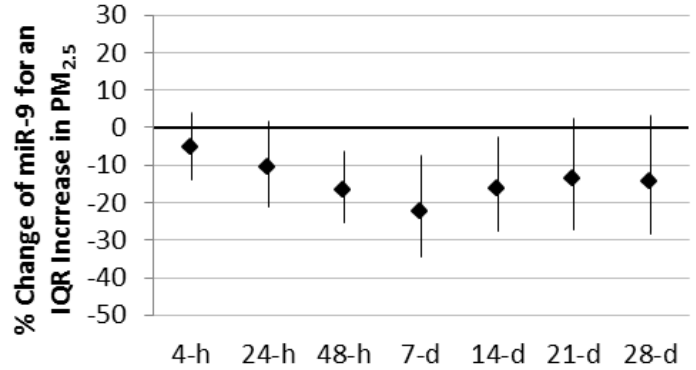
\includegraphics[height=12.em]{res_pm25}
  %      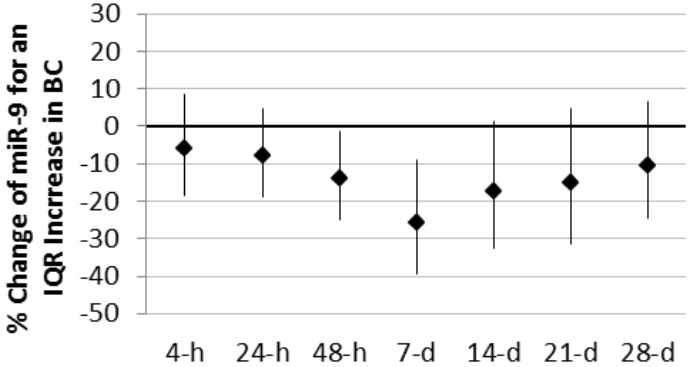
\includegraphics[height=12.em]{res_bc}
  %      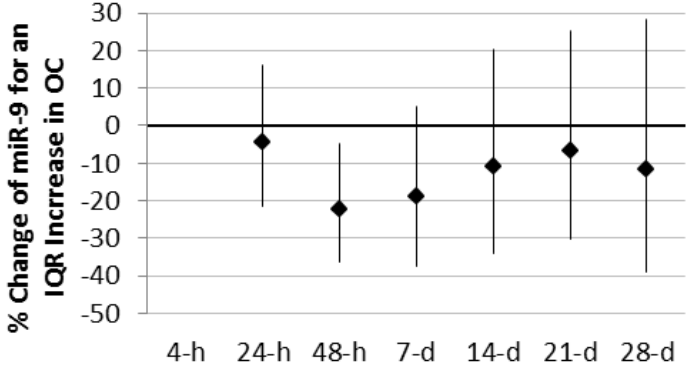
\includegraphics[height=12.em]{res_oc}
  %      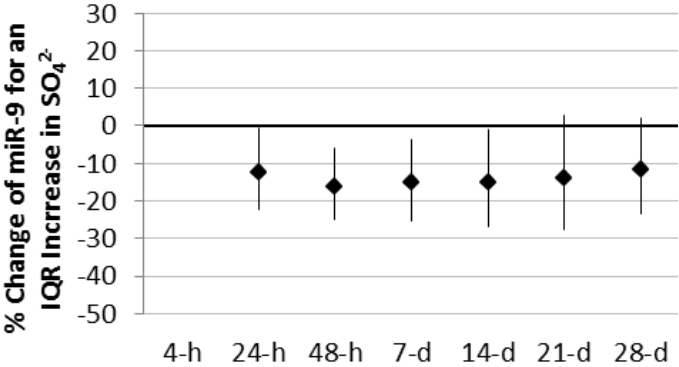
\includegraphics[height=12.em]{res_so}
  %   }
  % \begin{tabular*}{\linewidth}{*{5}{@{}p{0.7\linewidth}@{}}}
  %   {Figure C\hfill{}Figure D\hfill{}}
  % \end{tabular*}
  % \\[1em]
    
  \vspace{0.3em}
}
%%%%%%%%%%%%%%%%%%%%%%%%%%%%%%%%%%%%%%%%%%%%%%%%%%%%%%%%%%%%%%%%%%%%%%%%%%%%%%
  \headerbox{References}{name=references,column=3,above=bottom}{
%%%%%%%%%%%%%%%%%%%%%%%%%%%%%%%%%%%%%%%%%%%%%%%%%%%%%%%%%%%%%%%%%%%%%%%%%%%%%%
    \smaller
    \bibliographystyle{ieee}
    \renewcommand{\section}[2]{\vskip 0.05em}
    \nocite{*}
    \bibliography{biblio}
    %   \begin{thebibliography}{1}\itemsep=-0.01em
    %   \setlength{\baselineskip}{0.4em}
    %   \bibitem{amberg11:graphtrack}
    %     B.~Amberg, T. Vetter.
    %     \newblock {GraphTrack}: {F}ast and {G}lobally {O}ptimal {T}racking in {V}ideos
    %     \newblock In {\em CVPR '11}
    %   \bibitem{awf:tracking}
    %     A.~Buchanan and A.~Fitzgibbon.
    %     \newblock {I}nteractive {F}eature {T}racking using {K-D} {T}rees and {D}ynamic {P}rogramming.
    %     \newblock In {\em CVPR '06}
    %   \end{thebibliography}
    
   \vspace{0.3em}
  }

%%%%%%%%%%%%%%%%%%%%%%%%%%%%%%%%%%%%%%%%%%%%%%%%%%%%%%%%%%%%%%%%%%%%%%%%%%%%%%
\headerbox{Conclusion}{name=speed,column=3,span=1,below=future_works,above=references}{
  %%%%%%%%%%%%%%%%%%%%%%%%%%%%%%%%%%%%%%%%%%%%%%%%%%%%%%%%%%%%%%%%%%%%%%%%%%%%%%
  \indent Exposure to ambient particles could cause a downregulation of microRNAs involved in processes related to PM exposure, i.e. inflammation, vascular dysfunction and atherosclerosis.
  \\Open questions and plans.......
  \vspace{0.0em}
  }
%%%%%%%%%%%%%%%%%%%%%%%%%%%%%%%%%%%%%%%%%%%%%%%%%%%%%%%%%%%%%%%%%%%%%%%%%%%%%%
  \headerbox{Method}{name=method,column=1,row=0,span=2}{
%%%%%%%%%%%%%%%%%%%%%%%%%%%%%%%%%%%%%%%%%%%%%%%%%%%%%%%%%%%%%%%%%%%%%%%%%%%%%%
  \noindent
  \begin{tabular}{  p{1.6cm} p{13.cm} }
   {\bf Study \newline population} & \textbullet~153 elderly males from the Normative Aging Study \\
     & One visit between December 2005 and May 2007.\\    
    \hline
    {\bf Explosure} & \textbullet~Fine PM ($PM_{2.5}$), black carbon (BC), organic carbon (OC) and sulfates ($SO_4^{2-}$) measured at a stationary ambient monitoring site. Exposure in different time windows [4-hours to 28-days moving averages (MA)] \\
    \arrayrulecolor{blue}\hline
    {\bf Micro \newline RNAs} & \textbullet~We used stem-loop quantitative real-time RT-PCR to detect and quantify 14 miRNAs involved in processes related to systemic inflammation, endothelial dysfunction and atherosclerosis \\
    \arrayrulecolor{blue}\hline
    {\bf Statistical analysis}
    & \textbullet~Linear regression models, adjusted for age, body mass index (BMI), cigarette smoking (never, former, current), pack-years, percent of granulocytes, to control for possible shifts in leukocyte differential count, date, and seasonality (using sine and cosine), were used to assess effects of particles 
    \\ & \textbullet~Effect estimates ($\beta$) and their 95\% confidence intervals (CI) are presented as percent changes per interquartile range (IQR) change of pollutant at each averaging time period using the formula ($e^{\beta*IQR}$) × 100.
  \end{tabular}
   \vspace{0.3em}
  }

\headerbox{Deaths attributable to outdoor air pollution, 2008}{name=dead_map,column=1,row=0,span=2,below=method}{
  \noindent{\centering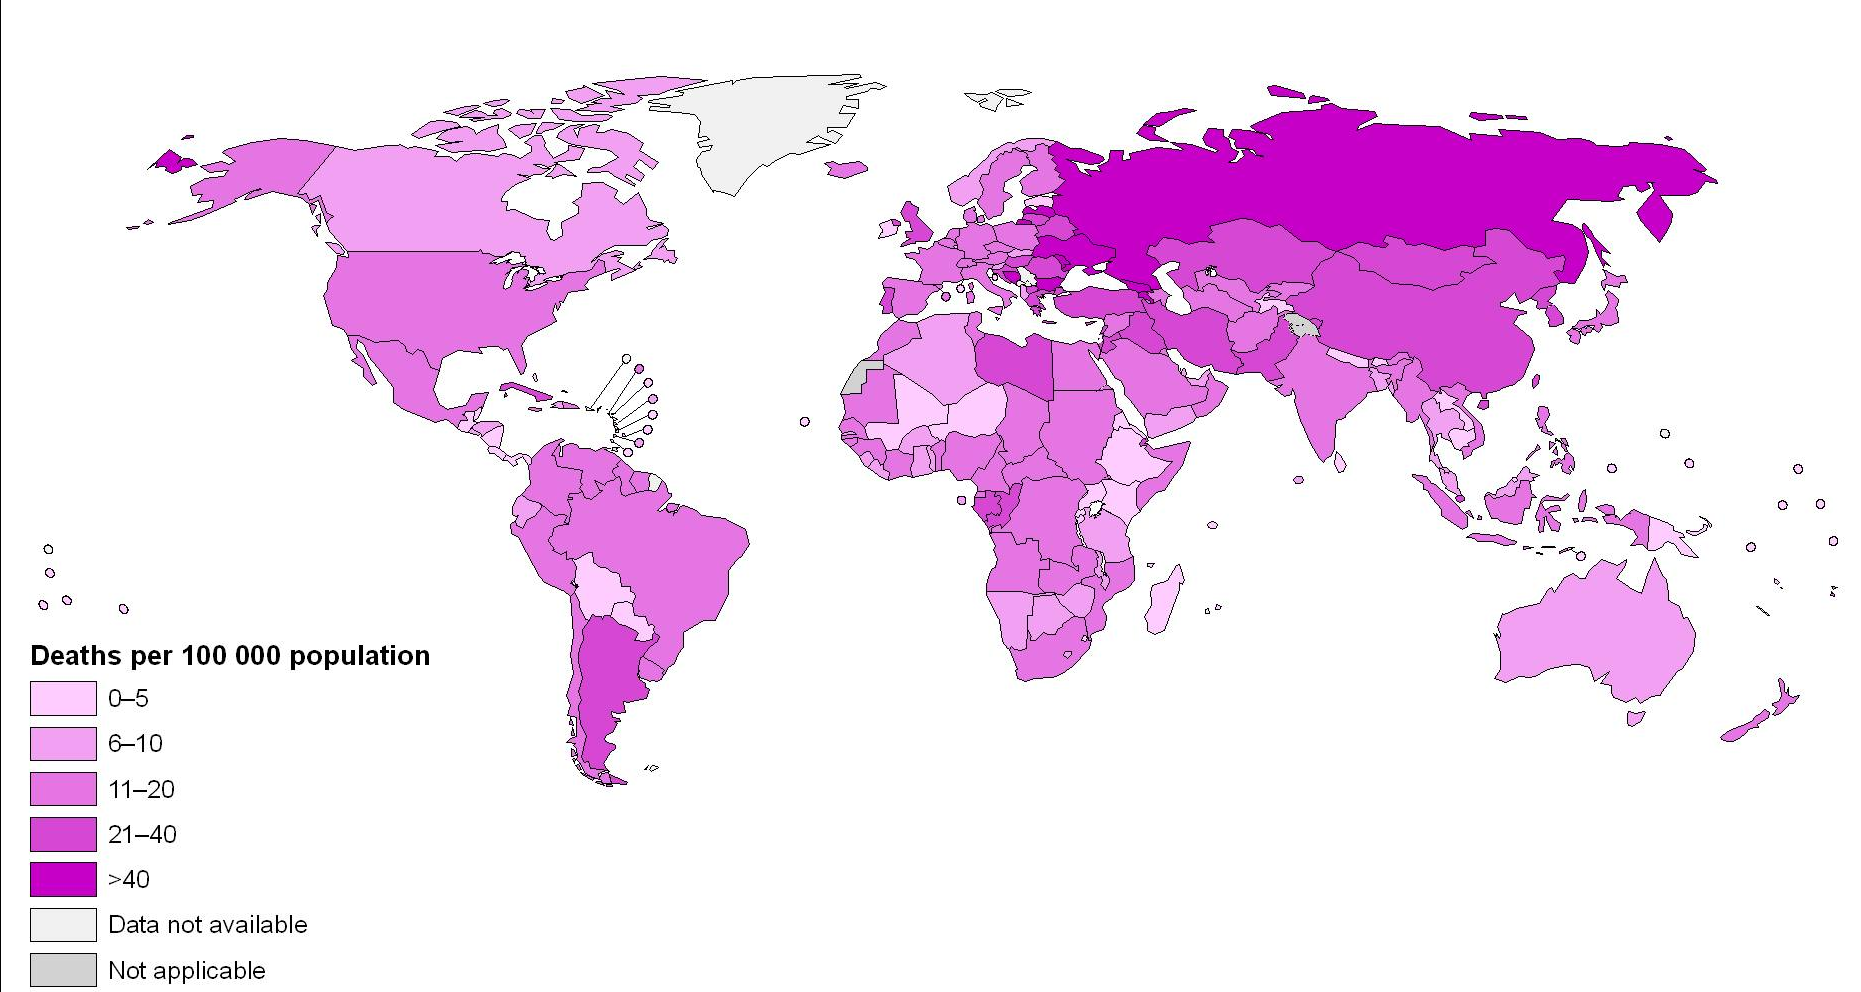
\includegraphics[width=0.95\linewidth]{air_pollution_map_min}}
}

\end{poster}

\end{document}